\scanpage{55}
\mspage{54}

majorées par $F$ s'appellent les \uline{strates} de $\deleted{E}F$. (Donc, \deleted{des} strate de $F$ est une multistrate)

L'ens des strates de $F$ \deleted{s'appelle} sera noté $\overline F$ : \[ \begin{aligned} \deleted{\overline F\subset M} &\qquad  M\subset\mathcal F\\ F\longrightarrow\overline F &\qquad \mathcal F\longrightarrow\mathcal P( M). \end{aligned} \]

\uline{$\mathcal C$ 2} Toute figure est la borne supérieure de ses strates : \[ F=\underset{\deleted{A}X\in\overline F}{\mathrm{Sup}}\ X \]
\figure{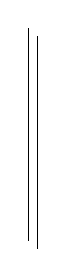
\begin{tikzpicture}\draw (0,0)--(0,2.7);\draw (.12,-.1)--(.12,2.6);\end{tikzpicture}}
\uline{Corollaire} 1 L'application $\deleted{X}F\longrightarrow\overline{\deleted{C}F}$ \[ \mathcal F\longrightarrow\mathcal P( M) \] est injection, et induit un iso d'ens ordonnés de $\mathcal F$ avec l'ens $\Phi\subset\mathcal P( M)$ formé des $\overline F$.

Cet iso. transforme $\underset{i}{\mathrm{Sup}}$ en $\bigcup_i$
\figure{\begin{tikzpicture}\draw (0,1.5)--(0,2.8);\draw (.1,-2)--(.1,.5);\end{tikzpicture}}
\uline{Corollaire 2} L'ens $\Phi$ des parties de $ M$ satisfont les deux conditions,

\deleted{a) $\Phi\ne\varnothing$}

% slanted
\margin{\deleted{Ceci}} \deleted{b)}a) Si $A\in\Phi$, et $(A_i)_{i\in\unsure{I|\Phi}}$ est une famille d'éléments de $\Phi$, avec $A_i\subset A$, alors $\bigcup_iA_i\in\Phi$.

b) $\forall X\in M$, il existe un plus petit $A=A_X$ tel que $X\in\unsure{A|A_x|A_X}$ (a fortiori, $\Phi$ recouvre $ M$).
